\documentclass[../document]{subfiles}

\begin{document}

\section{Conclusion}

\subsection{Introduction}
This section contains the system overview for the final draft of the project. It also includes further development plans for the project, or in other words, what could the project become in the future as well as any current project improvements. Finally, we briefly discuss testing and the overarching goal of the tests.

\subsection{System Overview}
The majority of the project was dedicated on completing the requirements set out by the customer. To that end planning, analysis of requirements and architecture, and three sprints were all focused on creating a fully functioning, modifiable prototype of our final product. However, in the latter part of the project we were tasked on adding additional features to our prototype, something that was not planned initially. The extra features do not use real data, but rather mock-up data, as we do not have the hardware to support these extra features. Therefore, we have constructed another prototype to accommodate these features into our original prototype. Each of the systems class diagrams can be seen in \figref{fig:ClassDiagramB} and {\color{red} (figure yet to be added)}.

\subsection{Hardware-Based Prototype}

\begin{figure}[H]
\centering
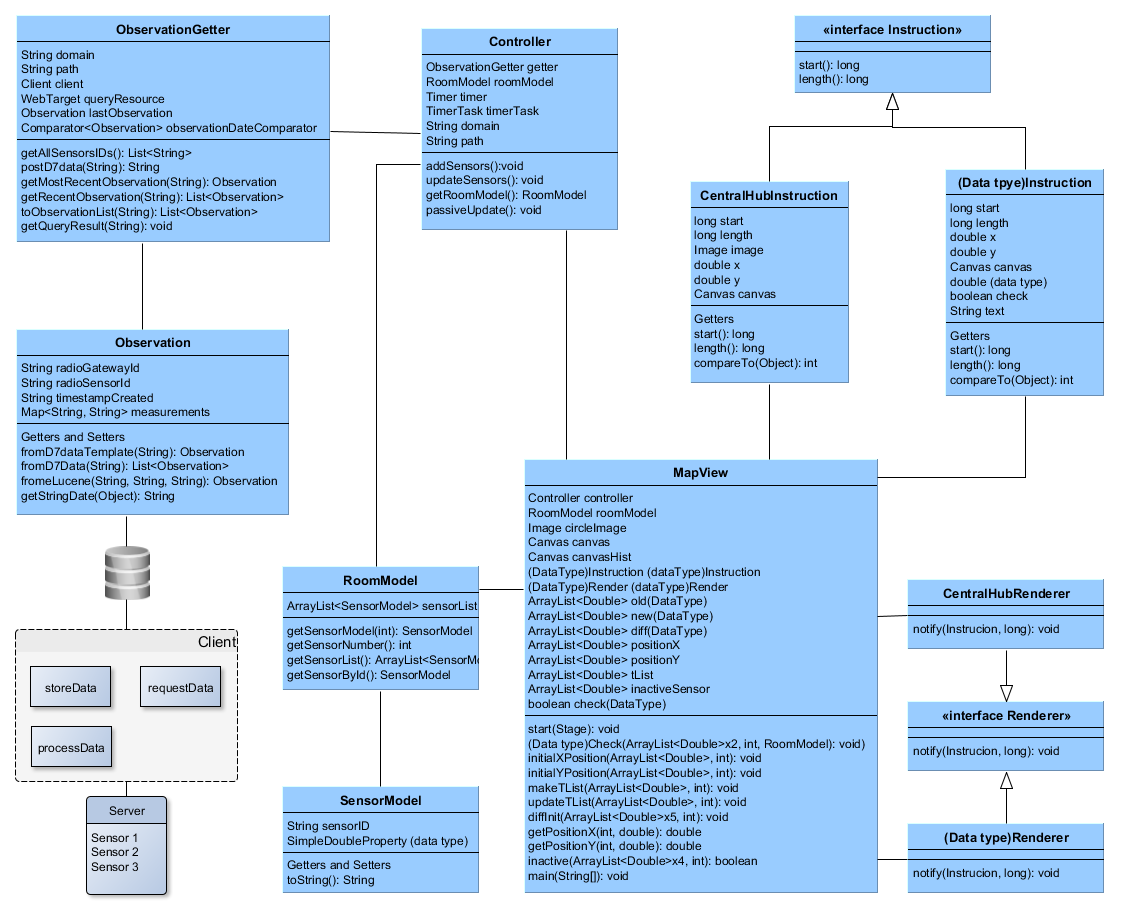
\includegraphics[width=\textwidth]{Architecture/ClassDiagramB.png}
\caption{Class Diagram for Hardware-based Prototype}
\label{fig:ClassDiagramB}
\end{figure}

The class diagram for the hardware-based, or real time prototype, shows how the classes interact with each other and the main methods and fields for each class. It also shows how the client requests data from the central hub and how the central hub gets the data from the sensors. The client then pushes the data into the database. The Controller uses a Timer to request data using methods in the ObservationGetter, then based on the data it gets, the Controller then creates or updates a list of SensorModels stored in a RoomModel object. The MapView is the class that is actually creating the visualisation by using a canvas and an animation timer. The animation timer updates the screen sixty frames per seconds. This frame rate can be adjusted to anything the customer would be pleased with, but the higher the frame rate, the smoother the animation. The animation timer uses Interfaces and Renderer classes to draw on the canvas and animate everything. The animation is done through events; every single time a value is changed an event fires off and the difference between the new and old values are calculated. This difference then is played over the time frame between the data pulls and it makes a smooth animation. 

Our class diagram has been scaled down, to make the image readable. Some fields and methods that are not really important are not included, and if a class has getters and setters, we have just indicated getters and setters, and did not mentioned them all. Constructors are not included as well, though many classes have a constructor method. Another difference is the places where the data types have methods and fields and classes that are similar have been merged together. An example is the instruction classes which we have written as (Datatype)Instruction, where (Datatype) is to be switched to either Temperature, Humidity, Pressure or Lighting. This is done to make it an easier and smaller class diagram. In the (Datatype)Instruction class the field String text is not in the HumidityInstruction nor in the PressureInstruction.

\subsection{Mock-Up Data Based Prototype}

{\color{red}This is going to be finished when the prototype C is finished. It is in the random crap document.}
\newline \ \newline
{\color{red}Class diagram image here}

Discussion

\subsection{Further Development}
A large part of future development for the project was already discussed in \sectionfullref{sec:preliminary_study}. This project is similar to an internal project carried out by a company. We do not do anything with the data but visualize it in an interesting fashion. As mentioned in \subfullref{subsec:initial_ideas}, we could use the data in health systems, exploration, high risk work environments as well as the smart room concept, for which we have quite a detailed set of requirements as well in \sectionfullref{sec:requirements_cast_1}. 

All of these systems, and many more could build on the base of this project. Furthermore, data visualisation is not completely useless. In a more advanced project, such as for example oil well digging, data visualisation is used with experts to determine if the system is behaving correctly. With substantial adjustments to our system, it too could potentially serve as a complex data visualisation system. These adjustments are, however, well beyond the scope of this project.

\subsection{Additional Improvement}
As we progressed through the project, we have discovered some limitations and as we approached the end of the project we have noted down several areas where both or either of the prototypes could be improved. The possible improvements are outlined in this section.

\subsubsection{Hardware Improvements}
The main field for improvement here are the sensors. From the first customer meeting, we were informed that the sensor manufacturer is not set in stone, and that we are required to make a system that will be independent of the sensor type. Still, the sensors that we received are the only real hardware that we worked with, so we will outline some of their limitations and improvements that could be looked into when developing the sensors. 

The first and major improvement is that could be done on the hardware is the ability to get correct data and that all of the data is recorded. In other words, we have found the sensors quite unreliable in most fields of measurement, except for lighting. Out of the two sensors, one had difficulty measuring temperature, humidity and pressure. The other sensor was able to measure temperature, but it had problems measuring humidity and pressure. Overall, from two sensors we can not get a correct impression, as both of the sensors electronics are unprotected and they have been shipped a long distance, from Oslo to Trondheim. They may, and most likely have, faults.

Secondly, while doing research on a specific value for the prototype with mock-up data we have discovered that it was quite inaccurate. The specific value in question is called the link budget. The link budget can be seen as the distance from the gateway to the sensors. The larger the link budget the larger the distance, and vice versa. However, we found the link budget to be quite lacking in accuracy. Not only is it quite inaccurate on distances, but it also has tremendous problems when faced with walls and other obstacles. The problem is not consistent enough for a solution on the front end. Instead, if precision is necessary, another system should be implemented instead of the link budget, or the link budget should be improved substantially. 

\subsubsection{Software Improvements}
A main improvement that the group was not concerned about, as it was low priority, is performance. Currently, while the simulation runs without any problems, it is not well optimized. It uses quite a lot of memory and processing power which could be reduced.

Another improvement that can be made is improving the look of the visualizer itself. None of us are graphics artists, and the visualisation is quite simple in it’s looks. It could be better looking, by adding effects such as shadows and drawing our sensors in a more aesthetically pleasing fashion. It could also be visualized in three dimensions, where we would be able to see the depth of the system as well. While this would definitely add complexity to the system, it would also mean that we could completely map an entire area and correctly show it as is.

Finally, our current software does not support every single value that the sensors can measure. Accelerometer values are not included in our visualisation, because of the difficulty of visualising them in two dimensions, as well as the lack of time to implement them correctly. Furthermore, as the data polling is every five seconds, accelerometer values could change drastically and be lost before the next poll. Sound is also one value that is not present on the sensors, but could be added with a different sensor manufacturer. Our software could be further improved by making functions that could take in more of these values and ignore them, should the sensors not have the capability of measuring them.

\subsection{Testing}
Most of the test were done at unit level by an individual team member, and we often used mock-up data to test the system with. The testing software was not a requirement from the customer side, and we felt that jUnit tests were not worth the time it would take to implement them. Instead, we used simple unit testing. Unit testing was useful since with it we had found most of the bugs in our system. This also gave us a high code coverage, and we made sure we had a 100\% state coverage in this way.

Integration testing was the most confusing part since the tools we were using were quite new for us. There were also changes in the backend during the project, therefore integration testing took quite a long time. Since we were only running a simple pull and push model, there were not that many bugs . Once we had all the components working and the connection was established in between them, we experienced only a handful of bugs. Most of the bugs here were related to the way we formatted the data.

Function testing was done at the end of sprint 3 and sprint 4, due to the nature of our program it was easy to perform once integration was working correctly. However we did experience some function loss due to hardware problems, therefore most of the tests were conducted with mock-up data.

With our tests we were trying to achieve the quality metrics that we set for ourselves in \subsubfullref{subsubsec:quality_metrics}. We often mention in tests that the group has to be agreed what a “smooth animation” should look like. We did not do any large-scale user testing due to the time and resources we had, however, we had included the adviser and the customer in our test results, which counts as a part of our unit testing. Performance and availability testing were done at the same time as functional testing. Test 4 from sprint 4 was aimed directly at performance and availability over a long period of time. 

\subsubsection{Testing Conclusion}
Our tests have been useful in uncovering bugs and problems with our system. Even more than that, the tests provided valuable data for future development, as we had directly tested the validity and precision of the sensors as well. We feel that the tests were quite useful, however, they did differ quite some from the initially planned tests. We also did not have any testers but us, although we did show the results to both the adviser and the customer and used their feedback to improve our system. 

\subsection{Summary}
The group was given a two-fold task. Think about what the internet of things is, and what it can be used for, and implement a showcase, that shows data received from sensors in a visually interesting fashion.

We have two prototypes, one that uses live data and one that uses mock-up data. The live data prototype visually shows the sensors orbiting a central hub. The sensors visualize the data with a combination of colors and geometrical shapes, with a legend on the right hand side explaining what each shape represents. The second prototype goes a step further, by adding the positional values in the system. This prototype uses mock-up data, and as such we can not demonstrate it with hardware. However, it should work exactly the same with hardware as it does with mock-up data. In the case of this prototype, the sensors do not move on their own. Instead, their position is calculated using trilateration, and drawn on the screen based on where they are in the room. Again, the same shapes and colours are used to represent different values that the sensors are measuring.

Overall, our customer was satisfied with the finished product. We believe that the product and the project served the customers needs, as it provided good research material for the customer. Furthermore, the project satisfies the needs set out it the project tasks as closely as possible, with the time given and with the changes introduced throughout the project.


\end{document}